\documentclass[a4paper]{article}

\usepackage[utf8]{inputenc} 
\usepackage{graphicx}

\title{Simulering av stjärnor i en galax}
\date{}

\begin{document}

	\maketitle


	\section{Översikt}

	I den här uppgifter kommer du att skriva ett program som simulerar hur
stjärnor rör sig i en galax. Metoden vi ska använda kallas N-body (som i N
stycken kroppar) och används i verktyg för att simulera riktiga fysikaliska
förlopp. I simuleringen skapar vi först ett antal stjärnor och placerar ut dem
på x- och y koordinater. Därefter börjar vi stega tiden framåt i små steg. I
varje tidssteg räknar vi ut åt vilket håll en stjärna dras åt och flyttar den.
Detta görs för alla stjärnor vilket exempelvis ger bilden nedan

	\begin{figure}[!h]
	\centering
	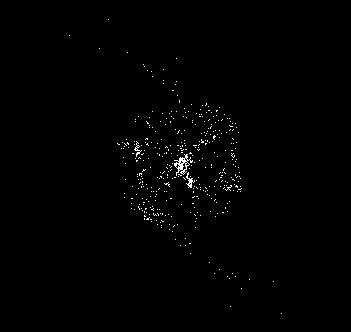
\includegraphics[scale=0.5]{galaxy.jpg}
	\caption{Uppgiften består av att skriva ett program som får stjärnorna att röra sig enligt Newtons gravitationslag. Med i koden finns en stomme för att rita upp stjärnorna som vita prickar i ett fönster}
	\end{figure}

	\section{Uppgiften}
	Du ska skriva ett program som simulerar stjärnornas rörelser enligt Newtons gravitationslag. Algoritmen som kommer att utstakas nedan heter N-body och gör att varje stjärna vet i vilken riktning den dras och hur st

	Programmet ska kunna ta emot två argumen

	
	\begin{verbatim}
		foo> ./galaxy ANTAL_STJÄRNOR ANTAL_ITERATIONER
	\end{verbatim}

	som ger antal stjärnor i simuleringen (STJÄRNOR) och antal tidssteg (ITERATIONER). 

	Två stjärnor, A och B, påverkar varandra en gravitationskraft enligt:

	$$ F_A = F_B = \frac{M_A*M_B}{r}*G $$

	där $F_A$,$F_B$ är kraften som verkar på A och B, $M_A$ $M_B$ är deras respektive massa, $r$ är avståndet mellan A och B och $G$ är en skumm konstant. Givet kraften, hur räknar vi ut stjärnans nya position? Att uppdatera stjärnans x-komponent ges av:

	$$a_x = F_X/M_X$$
	$$v_x = v_{x_0}+a_x*t$$
	$$x = x_{0} + v_{x_0}t+\frac{a_x*t^2}{2}$$

	p.s.s. för y-komponenten.

	En stjärna räknar ut summan av alla stjärnors påverkan för att bestämma sin nya koordinat. Detta görs enkelt i två loopar

	\begin{verbatim}
	// ett tidssteg
for star i in array_of_stars:
    for star j in array_of_stars:
        if i != j:
            star[i]->ax += compute_force_x(i,j);
            star[i]->ay += compute_force_y(i,j);

update_all_positions()
    \end{verbatim}

Uppgiften kan sammanfattas i några korta punkter:

\begin{itemize}
\item Skapa strukturen för en stjärna med poster för position,acceleration,fart mm.
\item Initiera alla stjärnor med en position och en initial fart.
\item Skriv tids-loopen, i-loopen,j-loopen och koden som räknar ut den nya kraften.
\item Skriv uppdateringsfunktionen.
\end{itemize}

\section{Kodskellet}

I kursrepot finns ett kodskellet för uppgiften. Det finns även ett byggskript
med två make-mål (\texttt{starsim} och \texttt{animate}). Det första målet
kompilerar koden; det andra målet kompilerar också koden men bygger även
med stöd för att visa en animaiton av simuleringen ni såg på bilden ovan. Animeringen fungerar bara om datorn ni använder stödjer X-fönsterservern. Animeringen har testats på IT-insitutionens maskiner. För att få animeringen att fungera på OS X behöver \texttt{gcc} hitta sökvägen till X-fönsterserverns header-filer och biblioteksfiler. 

Animationen kommer att fungera först när det finns stjärnor med x- och y-koordinater att visa.


\section{Bra att veta}

Skärmen är förinställd att vara 800 enheter bred och hög (800x800). Centrum för bilden ligger i punkten (400,400) eftersom (0,0) ligger i ett av hörnen. För att få en läcker spridning på stjärnorna kan deras först x och y-värde slumpas som ett tal mellan t.ex. 350 och 450 i både x- och y-riktningen




\end{document}
